\section*{Anhang}
\addcontentsline{toc}{section}{Anhang}
\label{sec:anhang}
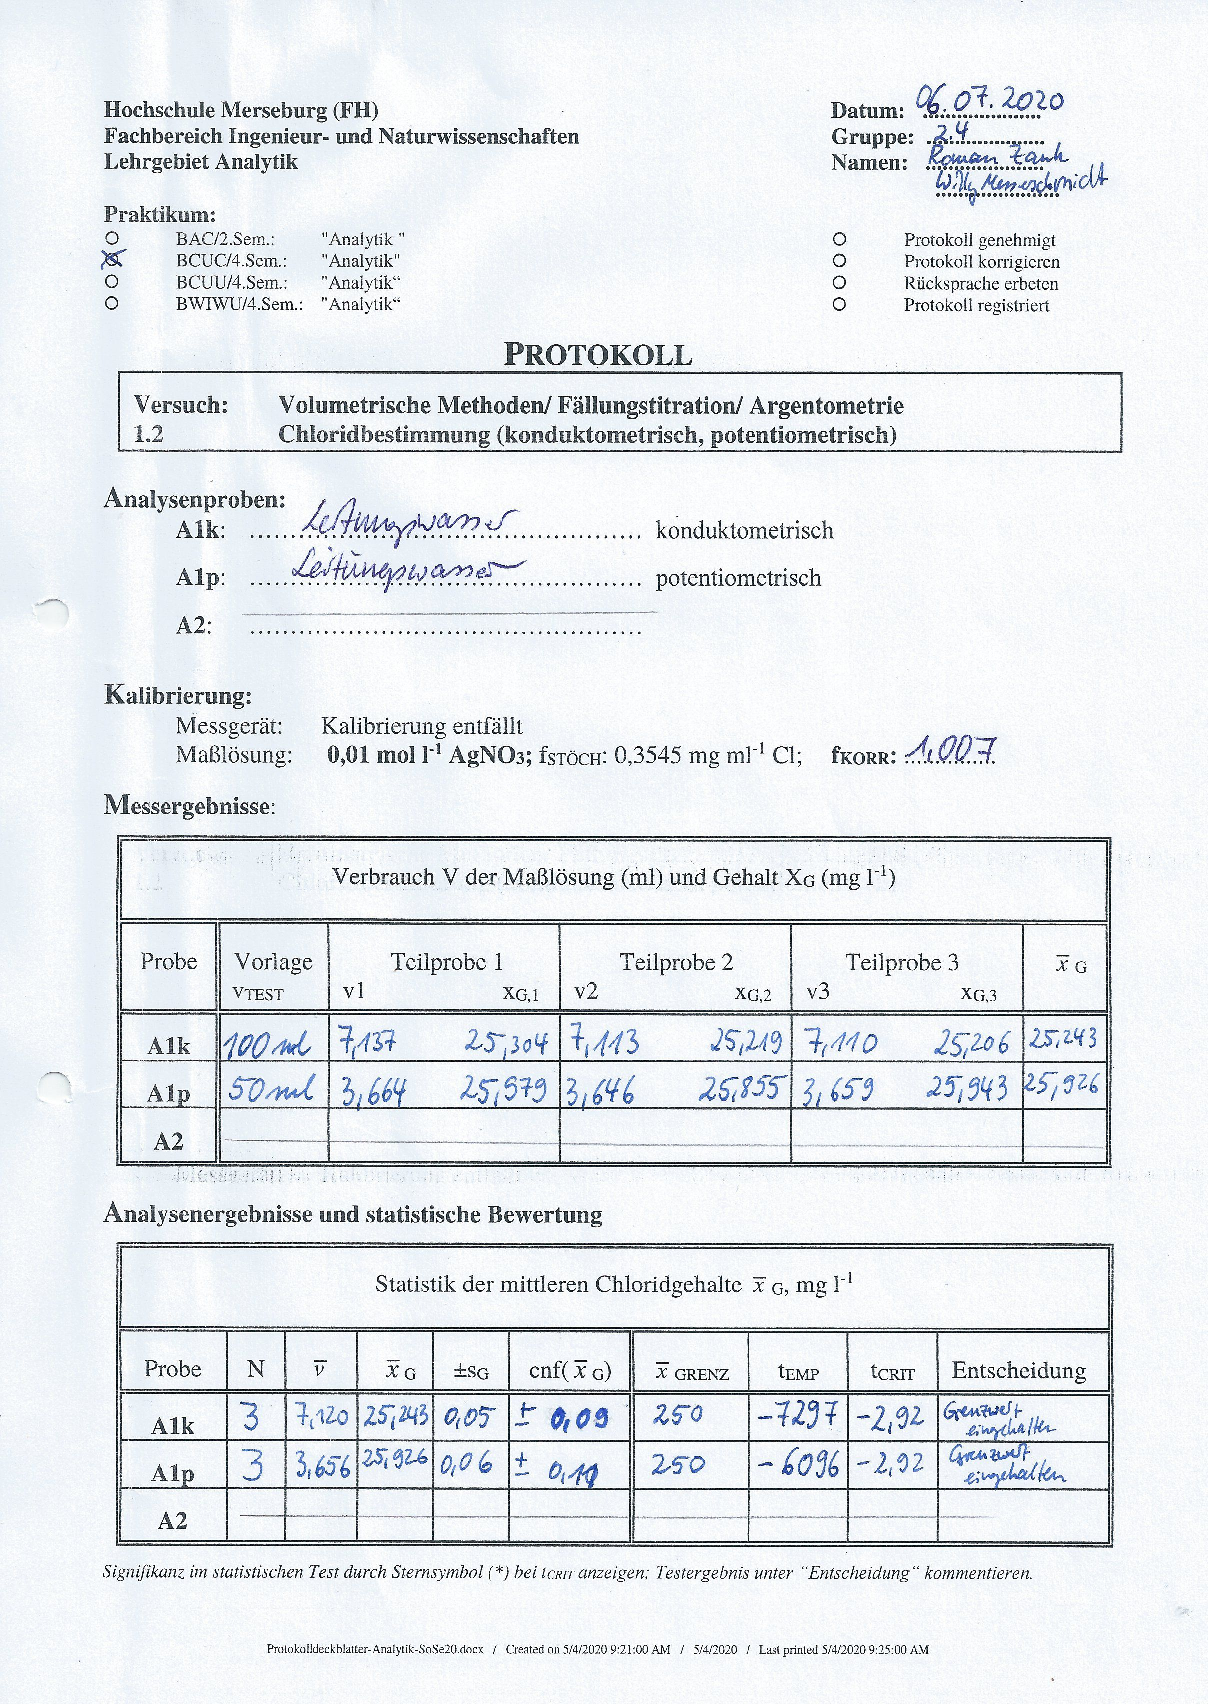
\includepdf[]{deckblatt.pdf}
\begin{table}[]
	\centering
	\caption{Messwerte Konduktometrie}
	\resizebox{!}{8cm}{
	\begin{tabular}{cc|cc|cc}
		\hline
		\multicolumn{2}{l}{\textbf{Messreihe 1}} & \multicolumn{2}{l}{\textbf{Messreihe 2}} & \multicolumn{2}{l}{\textbf{Messreihe 3}}  \\
		\hline
		0,0   & 545   & 0,0   & 545   & 0,0   & 543 \\
		0,5   & 543   & 0,5   & 544   & 0,5   & 541 \\
		1,0   & 540   & 1,0   & 541   & 1,0   & 538 \\
		1,5   & 537   & 1,5   & 538   & 1,5   & 535 \\
		2,0   & 534   & 2,0   & 535   & 2,0   & 533 \\
		2,5   & 532   & 2,5   & 533   & 2,5   & 530 \\
		3,0   & 529   & 3,0   & 530   & 3,0   & 528 \\
		3,5   & 526   & 3,5   & 527   & 3,5   & 525 \\
		4,0   & 524   & 4,0   & 525   & 4,0   & 522 \\
		4,5   & 521   & 4,5   & 522   & 4,5   & 520 \\
		5,0   & 518   & 5,0   & 520   & 5,0   & 518 \\
		5,5   & 516   & 5,5   & 517   & 5,5   & 515 \\
		6,0   & 514   & 6,0   & 515   & 6,0   & 513 \\
		6,5   & 511   & 6,5   & 513   & 6,5   & 511 \\
		7,0   & 510   & 7,0   & 511   & 7,0   & 509 \\
		7,5   & 512   & 7,5   & 514   & 7,5   & 512 \\
		8,0   & 518   & 8,0   & 520   & 8,0   & 519 \\
		8,5   & 526   & 8,5   & 528   & 8,5   & 526 \\
		9,0   & 533   & 9,0   & 535   & 9,0   & 534 \\
		9,5   & 540   & 9,5   & 543   & 9,5   & 541 \\
		10,0  & 548   & 10,0  & 551   & 10,0  & 549 \\
		10,5  & 555   & 10,5  & 558   & 10,5  & 556 \\
		11,0  & 563   & 11,0  & 565   & 11,0  & 564 \\
		11,5  & 570   & 11,5  & 573   & 11,5  & 571 \\
		12,0  & 577   & 12,0  & 580   & 12,0  & 579 \\
		12,5  & 585   & 12,5  & 587   & 12,5  & 586 \\
		13,0  & 592   & 13,0  & 595   & 13,0  & 593 \\
		13,5  & 599   & 13,5  & 602   & 13,5  & 600 \\
		14,0  & 606   & 14,0  & 609   & 14,0  & 607 \\
		14,5  & 613   & 14,5  & 616   & 14,5  & 614 \\
		15,0  & 620   & 15,0  & 623   & 15,0  & 621 \\
		15,5  & 626   & 15,5  & 630   & 15,5  & 628 \\
		16,0  & 633   & 16,0  & 636   & 16,0  & 635 \\
		16,5  & 640   & 16,5  & 643   & 16,5  & 642 \\
		17,0  & 647   & 17,0  & 650   & 17,0  & 649 \\
		17,5  & 653   & 17,5  & 657   & 17,5  & 655 \\
		18,0  & 660   & 18,0  & 663   & 18,0  & 662 \\
		18,5  & 666   & 18,5  & 670   & 18,5  & 669 \\
		19,0  & 673   & 19,0  & 676   & 19,0  & 675 \\
		19,5  & 679   & 19,5  & 683   & 19,5  & 682 \\
		20,0  & 685   & 20,0  & 689   & 20,0  & 688 
	\end{tabular}}
	\label{tab:kondu_mess}%
\end{table}%
\FloatBarrier
\begin{table}[h!]
	\centering
	\caption{Messwerte Konduktometrie}
	\begin{tabular}{ccc|ccc|ccc}
		\hline
	\multicolumn{2}{l}{\textbf{Messreihen 1}} &       \multicolumn{1}{l}{$\Delta E_1$} & \multicolumn{2}{l}{\textbf{Messreihen 2}} &        \multicolumn{1}{l}{$\Delta E_2$} & \multicolumn{2}{l}{\textbf{Messreihen 3}} & \multicolumn{1}{l}{$\Delta E_3$} \\
	\hline
	0,0   & 174   & - & 0,0   & 186   & - & 0,0   & 186   & -\\
	0,5   & 182   & 8     & 0,5   & 189   & 3     & 0,5   & 189   & 3 \\
	1,0   & 187   & 5     & 1,0   & 194   & 5     & 1,0   & 193   & 4 \\
	1,5   & 192   & 5     & 1,5   & 199   & 5     & 1,5   & 198   & 5 \\
	2,0   & 199   & 7     & 2,0   & 205   & 6     & 2,0   & 204   & 6 \\
	2,5   & 207   & 8     & 2,5   & 215   & 10    & 2,5   & 213   & 9 \\
	3,0   & 220   & 13    & 3,0   & 228   & 13    & 3,0   & 226   & 13 \\
	3,5   & 245   & 25    & 3,5   & 256   & 28    & 3,5   & 251   & 25 \\
	4,0   & 301   & 56    & 4,0   & 307   & 51    & 4,0   & 304   & 53 \\
	4,5   & 326   & 25    & 4,5   & 328   & 21    & 4,5   & 328   & 24 \\
	5,0   & 339   & 13    & 5,0   & 340   & 12    & 5,0   & 340   & 12 \\
	5,5   & 347   & 8     & 5,5   & 348   & 8     & 5,5   & 347   & 7 \\
	6,0   & 354   & 7     & 6,0   & 354   & 6     & 6,0   & 353   & 6 \\
	6,5   & 358   & 4     & 6,5   & 358   & 4     & 6,5   & 358   & 5 \\
	7,0   & 362   & 4     & 7,0   & 362   & 4     & 7,0   & 361   & 3 \\
	7,5   & 366   & 4     & 7,5   & 365   & 3     & 7,5   & 365   & 4 \\
	8,0   & 369   & 3     & 8,0   & 368   & 3     & 8,0   & 367   & 2 \\
	8,5   & 371   & 2     & 8,5   & 371   & 3     & 8,5   & 370   & 3 \\
	9,0   & 374   & 3     & 9,0   & 373   & 2     & 9,0   & 372   & 2 \\
	9,5   & 375   & 1     & 9,5   & 375   & 2     & 9,5   & 374   & 2 \\
	10,0  & 377   & 2     & 10,0  & 377   & 2     & 10,0  & 376   & 2 
\end{tabular}%
\label{tab:potentio_mess}
\end{table}
\FloatBarrier

